\documentclass[11pt,a4paper]{article}

% Packages
\usepackage[utf8]{inputenc}
\usepackage[T1]{fontenc}

\usepackage{geometry}
\usepackage{hyperref}
\usepackage{xcolor}
\usepackage{amsmath,amssymb}
\usepackage{array}
\usepackage{booktabs}
\usepackage{longtable}
\usepackage{tabularx}
\usepackage{enumitem}
\usepackage{float}
\usepackage{caption}
\usepackage{subcaption}
\usepackage{listings}
\usepackage{fancyhdr}
\usepackage{titlesec}
\usepackage{tcolorbox}
\usepackage{tikz}
\usepackage{tikz-cd}
\usetikzlibrary{arrows.meta,positioning,shapes.geometric,shapes.multipart,fit,backgrounds,calc}

\geometry{left=1in,right=1in,top=1.0in,bottom=1.0in}

% Colors
\definecolor{deepblue}{HTML}{16324F}
\definecolor{midblue}{HTML}{2B5C88}
\definecolor{lightblue}{HTML}{3A7CA5}
\definecolor{softblue}{HTML}{EAF3FA}
\definecolor{softgreen}{HTML}{E9F6EC}
\definecolor{softyellow}{HTML}{FFF8E1}
\definecolor{softred}{HTML}{FDECEC}
\definecolor{softgray}{HTML}{F6F7F9}
\definecolor{darkgray}{HTML}{333333}
\definecolor{codebg}{HTML}{F7F7F7}
\definecolor{coderule}{HTML}{D9DDE3}
\definecolor{promptbg}{HTML}{F0F4FF}
\definecolor{promptframe}{HTML}{4A6FA5}

% Section formatting
\titleformat{\section}{\Large\bfseries\color{deepblue}}{\thesection}{0.8em}{}
\titleformat{\subsection}{\large\bfseries\color{midblue}}{\thesubsection}{0.8em}{}
\titleformat{\subsubsection}{\normalsize\bfseries\color{lightblue}}{\thesubsubsection}{0.8em}{}

% Header / footer
\pagestyle{fancy}
\fancyhf{}
\fancyhead[L]{\small\textit{Orthosolver NL Pipeline Architecture v2.1}}
\fancyhead[R]{\small\textit{Orchestrator \& Natural-Language Agents}}
\fancyfoot[C]{\small\thepage}
\renewcommand{\headrulewidth}{0.4pt}

% Hyperlinks
\hypersetup{
  colorlinks=true,
  linkcolor=deepblue,
  citecolor=deepblue,
  urlcolor=lightblue
}

% tcolorbox
\tcbuselibrary{skins,breakable}
\newtcolorbox{mustbox}[1][] {colback=softred,colframe=red!60!black,fonttitle=\bfseries,title=#1,arc=2mm,boxrule=0.8pt,breakable}
\newtcolorbox{notebox}[1][] {colback=softblue,colframe=deepblue,fonttitle=\bfseries,title=#1,arc=2mm,boxrule=0.8pt,breakable}
\newtcolorbox{goodbox}[1][] {colback=softgreen,colframe=green!50!black,fonttitle=\bfseries,title=#1,arc=2mm,boxrule=0.8pt,breakable}
\newtcolorbox{policybox}[1][] {colback=softyellow,colframe=orange!70!black,fonttitle=\bfseries,title=#1,arc=2mm,boxrule=0.8pt,breakable}
\newtcolorbox{promptbox}[1][] {colback=promptbg,colframe=promptframe,fonttitle=\bfseries\color{white},colbacktitle=promptframe,title=#1,arc=2mm,boxrule=0.8pt,breakable}

% Listings for JSON
\lstdefinelanguage{json}{
  basicstyle=\ttfamily\small,
  numbers=left,
  numberstyle=\tiny\color{gray},
  stepnumber=1,
  numbersep=8pt,
  showstringspaces=false,
  breaklines=true,
  frame=single,
  rulecolor=\color{coderule},
  backgroundcolor=\color{codebg},
  literate=
   *{0}{{{0}}}{1}
    {1}{{{1}}}{1}
    {2}{{{2}}}{1}
    {3}{{{3}}}{1}
    {4}{{{4}}}{1}
    {5}{{{5}}}{1}
    {6}{{{6}}}{1}
    {7}{{{7}}}{1}
    {8}{{{8}}}{1}
    {9}{{{9}}}{1}
    {:}{{{\color{black}{:}}}}{1}
    {,}{{{\color{black}{,}}}}{1}
    {\{}{{{\color{black}{\{}}}}{1}
    {\}}{{{\color{black}{\}}}}}{1}
    {[}{{{\color{black}{[}}}}{1}
    {]}{{{\color{black}{]}}}}{1},
  morestring=[b]",
  stringstyle=\color{midblue},
  commentstyle=\color{gray},
  keywordstyle=\color{deepblue}\bfseries
}

\lstdefinelanguage{prompt}{
  basicstyle=\ttfamily\small,
  showstringspaces=false,
  breaklines=true,
  frame=none,
  backgroundcolor=\color{promptbg},
  columns=flexible
}

\lstdefinelanguage{sql}{
  basicstyle=\ttfamily\small,
  numbers=left,
  numberstyle=\tiny\color{gray},
  stepnumber=1,
  numbersep=8pt,
  showstringspaces=false,
  breaklines=true,
  frame=single,
  rulecolor=\color{coderule},
  backgroundcolor=\color{codebg},
  keywords={CREATE,TABLE,IF,NOT,EXISTS,PRIMARY,KEY,REFERENCES,DEFAULT,CHECK,UNIQUE,INDEX,ON,TEXT,INTEGER,BOOLEAN,REAL,TIMESTAMP,JSONB,NULL,WITH,TIME,ZONE,NOW,SERIAL,BIGSERIAL,VARCHAR,ENUM,TYPE,AS,CONSTRAINT,FOREIGN,CASCADE,SET,USING,BTREE,GIN,BIGINT,GENERATED,ALWAYS,IDENTITY,SMALLINT},
  keywordstyle=\color{deepblue}\bfseries,
  morestring=[b]',
  stringstyle=\color{midblue},
  morecomment=[l]{--},
  commentstyle=\color{gray}\itshape,
  columns=flexible
}

\lstdefinelanguage{hcl}{
  basicstyle=\ttfamily\small,
  numbers=left,
  numberstyle=\tiny\color{gray},
  stepnumber=1,
  numbersep=8pt,
  showstringspaces=false,
  breaklines=true,
  frame=single,
  rulecolor=\color{coderule},
  backgroundcolor=\color{codebg},
  keywords={resource,variable,output,data,locals,module,provider,terraform,required_providers,backend,for_each,count,depends_on,lifecycle,dynamic,content},
  keywordstyle=\color{deepblue}\bfseries,
  morestring=[b]",
  stringstyle=\color{midblue},
  morecomment=[l]{\#},
  morecomment=[s]{/*}{*/},
  commentstyle=\color{gray}\itshape,
  columns=flexible
}

\lstset{language=json}

\newcommand{\Lean}{\textsc{Lean}}
\newcommand{\Vertex}{Vertex AI}
\newcommand{\Claude}{Claude}

\begin{document}

\begin{titlepage}
\centering
\vspace*{1.6cm}

{\Huge\bfseries\color{deepblue} Orthosolver NL Pipeline \\[0.3cm] Architecture Specification}

\vspace{0.8cm}

{\Large\color{midblue} Orchestrator, Natural-Language Agents, Database, \\[0.15cm] and Infrastructure}

\vspace{0.7cm}
\rule{0.75\textwidth}{1pt}

\vspace{1.0cm}

{\large Implementation Specification for the Orchestrator Engineer}

\vspace{0.4cm}

{\normalsize Version 2.1 \\ March 2026}

\vspace{1.5cm}

\begin{abstract}
\noindent This document specifies the complete architecture of the Orthosolver natural-language pipeline: the orchestrator that drives the proof search, the five NL agents (semantic sketch generator, decomposer, decomposition vetter, lemma solver, lemma proof vetter), the controller state machine and routing policy, the persistent data model and relational database schema, the public API, the NL-only operating mode, and the GCP infrastructure managed via Terraform. This document also specifies the complete HTTP API contract for the \Lean{} engine so the orchestrator can call it correctly, but it does \textbf{not} specify the \Lean{} engine's internal implementation (repair loop, \Claude{} agent, Docker build). That is covered in the companion document: \textit{Orthosolver Lean Engine Architecture Specification}.
\end{abstract}

\vfill

{\small Companion document: \textit{Orthosolver Lean Engine Architecture Specification v2.1}}
\end{titlepage}

\tableofcontents
\newpage

%% ═══════════════════════════════════════════════════════════════════════════════
\section{Purpose, Audience, and Scope}
%% ═══════════════════════════════════════════════════════════════════════════════

This document is for the engineer implementing the orchestrator, NL agents, database layer, public API, and GCP infrastructure. It contains everything needed to build, test, and deploy the NL pipeline independently of the \Lean{} engine.

\subsection{What This Document Covers}
\begin{itemize}[leftmargin=2em]
  \item End-to-end NL pipeline architecture and component responsibilities.
  \item All persistent data objects and their fields.
  \item Complete PostgreSQL relational schema (DDL).
  \item Controller state machine and all routing tables.
  \item Complete agent prompt specifications for Agents 1--5 and Agent 7 (statement plausibility checker prompt, which runs inside the \Lean{} engine but whose invocation the orchestrator controls).
  \item NL-only mode: full specification and mode-switching semantics.
  \item The \Lean{} engine HTTP API contract (what you call, what you receive back).
  \item Mock \Lean{} engine service for development without the real engine.
  \item Public orchestrator API.
  \item GCP deployment with complete Terraform IaC.
\end{itemize}

\subsection{What This Document Does \textbf{Not} Cover}
\begin{itemize}[leftmargin=2em]
  \item The \Lean{} engine's internal repair loop and conversation management.
  \item Agent 6 (the \Claude{} formalization agent running inside the \Lean{} engine).
  \item The \Lean{} Docker image build process and Mathlib compilation.
  \item \Lean{} engine internal architecture and scaling.
\end{itemize}
These are specified in the companion document: \textit{Orthosolver Lean Engine Architecture Specification}.

%% ═══════════════════════════════════════════════════════════════════════════════
\section{System Goals and Non-Negotiable Principles}
%% ═══════════════════════════════════════════════════════════════════════════════

\subsection{Primary Goal}
Given a target theorem, produce a fully formalized \Lean{} theorem and proof accepted by the \Lean{} kernel, with no \texttt{sorry}, no \texttt{admit}, and no trusted fake theorem injection.

\subsection{Non-Negotiable Principles}

\begin{mustbox}[Ground-Truth Principle]
A theorem or lemma counts as proved only if the final formalization compiles in \Lean{} and passes all system proof-validity checks. Natural-language acceptance is never sufficient for final correctness. \textbf{Exception:} when \texttt{nl\_only\_mode} is enabled (Section~\ref{sec:nl_only_mode}), vetter acceptance is treated as the terminal success criterion. Results produced under NL-only mode carry no formal verification guarantee and are explicitly tagged as such.
\end{mustbox}

\begin{policybox}[Trusted Context Principle]
Only already-formalized and compiler-accepted declarations may enter the system's reusable formal context. Natural-language claims, plausible claims, or LLM-vetted claims do not enter trusted context until they have been formalized and verified by the \Lean{} compiler.
\end{policybox}

\begin{policybox}[Separation of Concerns]
The natural-language pipeline is responsible for search, decomposition, natural-language proving, and natural-language vetting. The \Lean{} engine is responsible for formalization, compilation, repair, and final fatal-vs-repairable classification from the formal side. The \Lean{} engine is the sole authority on whether a failure is mathematical or a formalization artifact.
\end{policybox}

\begin{policybox}[Semantic Consistency Principle]
Every theorem and lemma carries a structured semantic sketch generated at creation time. Every vetter checks the current object's semantic sketch against the root theorem's immutable semantic sketch and flags any material drift. Major drift is a hard stop.
\end{policybox}

\begin{policybox}[Root Theorem Naming]
The root objective is the only object of kind \texttt{theorem}. Every non-root proof obligation is a \texttt{lemma}, even if produced late by recursive decomposition.
\end{policybox}

\begin{policybox}[Trivial Assembly Principle]
The assembly plan must consist only of trivial composition of already-proved lemmas. The assembly proof in \Lean{} must contain no non-trivial intermediate steps. Any intermediate claim requiring non-trivial reasoning must be surfaced as an explicit named lemma at decomposition time. This is a hard constraint on the decomposer.
\end{policybox}

\begin{policybox}[No Hardcoded Limits]
No retry count, depth limit, timeout, or budget is hardcoded in any service. All limits are read from the problem's configuration object at runtime. Services must respect the configuration they receive and must not apply internal overrides.
\end{policybox}

\subsection{Secondary Goals}
\begin{itemize}[leftmargin=2em]
  \item Minimize wasted \Lean{} formalization on obviously bad natural-language proofs.
  \item Make all routing decisions explicit and inspectable.
  \item Make services independently deployable and testable.
  \item Allow parallel execution across decompositions and lemmas.
\end{itemize}

%% ═══════════════════════════════════════════════════════════════════════════════
\section{High-Level System Overview}
%% ═══════════════════════════════════════════════════════════════════════════════

At a high level, the system executes the following loop (under standard mode; see Section~\ref{sec:nl_only_mode} for the NL-only variant):

\begin{enumerate}[leftmargin=2em]
  \item Accept a theorem submission. Generate a semantic sketch for the root theorem. Store it as immutable.
  \item Generate up to two decomposition candidates in natural language; each lemma carries its own semantic sketch.
  \item Vet each decomposition: check individual lemmas, assembly skeleton, coverage, and drift against the root semantic sketch.
  \item Run \Lean{} assembly-checks in parallel for surviving decompositions. Pin statement signatures from the assembly check.
  \item Select one active decomposition (lowest formalization cost estimate among assembly-check winners). Place the other in standby.
  \item For the active decomposition, solve open lemmas in natural language in parallel.
  \item Vet each lemma proof. Route based on gap severity and drift status.
  \item Send approved lemmas to the \Lean{} engine for formalization using pinned statement signatures.
  \item On \Lean{} success, add the resulting declaration to trusted formal context.
  \item When all lemmas for the active decomposition are formalized, run \texttt{assemble\_root}.
  \item If the active decomposition fails terminally, promote the standby decomposition if available.
  \item Continue until the root theorem compiles or the controller exhausts configured policy limits.
\end{enumerate}

\begin{figure}[H]
\centering
\resizebox{\textwidth}{!}{%
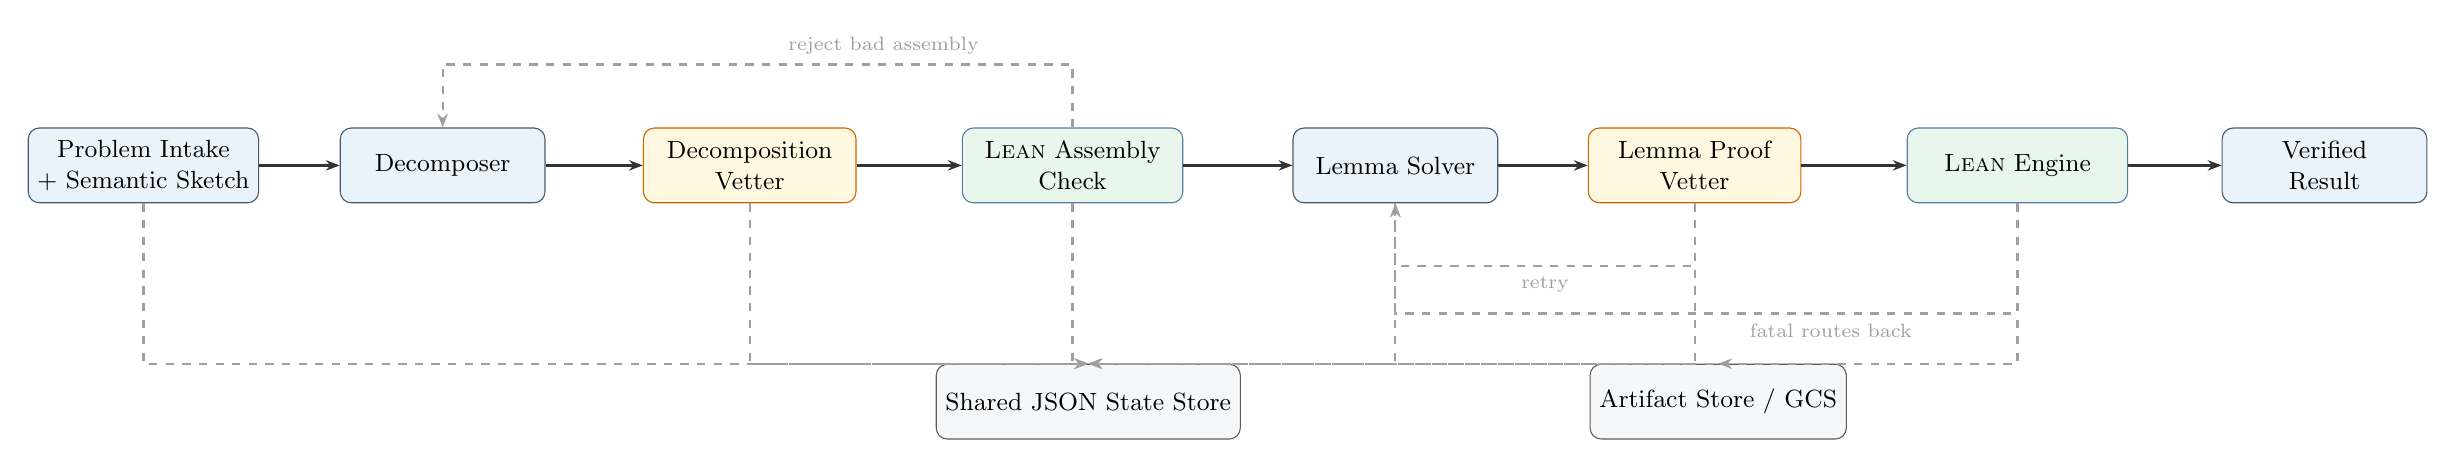
\begin{tikzpicture}[
  every node/.style={font=\small},
  comp/.style={rectangle,rounded corners=4pt,draw=deepblue!80,fill=softblue,minimum width=2.6cm,minimum height=0.95cm,align=center},
  aux/.style={rectangle,rounded corners=4pt,draw=midblue!80,fill=softgreen,minimum width=2.8cm,minimum height=0.95cm,align=center},
  err/.style={rectangle,rounded corners=4pt,draw=orange!80!black,fill=softyellow,minimum width=2.7cm,minimum height=0.95cm,align=center},
  db/.style={rectangle,rounded corners=4pt,draw=darkgray!80,fill=softgray,minimum width=2.8cm,minimum height=0.95cm,align=center},
  arrow/.style={-{Stealth[length=5pt]},thick,color=darkgray},
  dashedarrow/.style={-{Stealth[length=5pt]},thick,dashed,color=gray!75}
]

\node[comp] (submit) at (0,0) {Problem Intake\\+ Semantic Sketch};
\node[comp] (decomp) at (3.8,0) {Decomposer};
\node[err]  (dvet) at (7.7,0) {Decomposition\\Vetter};
\node[aux]  (acheck) at (11.8,0) {\Lean{} Assembly\\Check};
\node[comp] (solve) at (15.9,0) {Lemma Solver};
\node[err]  (lvet) at (19.7,0) {Lemma Proof\\Vetter};
\node[aux]  (lean) at (23.8,0) {\Lean{} Engine};
\node[comp] (done) at (27.7,0) {Verified\\Result};

\node[db] (state) at (12,-3.0) {Shared JSON State Store};
\node[db] (gcs) at (20,-3.0) {Artifact Store / GCS};

\draw[arrow] (submit) -- (decomp);
\draw[arrow] (decomp) -- (dvet);
\draw[arrow] (dvet) -- (acheck);
\draw[arrow] (acheck) -- (solve);
\draw[arrow] (solve) -- (lvet);
\draw[arrow] (lvet) -- (lean);
\draw[arrow] (lean) -- (done);

\draw[dashedarrow] (dvet.south) |- (state.north);
\draw[dashedarrow] (acheck.south) |- (state.north);
\draw[dashedarrow] (solve.south) |- (state.north);
\draw[dashedarrow] (lvet.south) |- (state.north);
\draw[dashedarrow] (lean.south) |- (state.north);
\draw[dashedarrow] (lean.south) |- (gcs.north);
\draw[dashedarrow] (submit.south) |- (state.north);

\draw[dashedarrow] (lvet.south) -- ++(0,-0.8) -| (solve.south) node[pos=0.25,below,font=\scriptsize] {retry};
\draw[dashedarrow] (acheck.north) -- ++(0,0.8) -| (decomp.north) node[pos=0.15,above,font=\scriptsize] {reject bad assembly};
\draw[dashedarrow] (lean.south) -- ++(0,-1.4) -| (solve.south) node[pos=0.15,below,font=\scriptsize] {fatal routes back};
\end{tikzpicture}%
}
\caption{Top-level component flow. Green boxes are \Lean{} engine calls (skipped in NL-only mode). The controller persists every state transition and artifact.}
\end{figure}

%% ═══════════════════════════════════════════════════════════════════════════════
\section{Natural-Language-Only Mode}
\label{sec:nl_only_mode}
%% ═══════════════════════════════════════════════════════════════════════════════

When \texttt{config.mode.nl\_only\_mode} is set to \texttt{true}, the system operates as a \textbf{pure natural-language reasoner} with no communication with the \Lean{} engine whatsoever. This is a runtime toggle in the problem configuration, identical in mechanism to every other setting in Section~\ref{sec:config}.

\subsection{Motivation}
\begin{itemize}[leftmargin=2em]
  \item \textbf{Fast exploratory runs.} Evaluate decomposition quality, solver strength, and vetter accuracy without \Lean{} build costs or latency.
  \item \textbf{NL-pipeline development.} Iterate on Agents~1--5 without deploying or depending on the \Lean{} engine infrastructure.
  \item \textbf{Benchmarking.} Score the NL pipeline against known results to calibrate vetter thresholds before formal verification is enabled.
\end{itemize}

\subsection{Behavioral Changes}

\begin{policybox}[NL-Only Mode: Pipeline Bypass Rules]
When \texttt{nl\_only\_mode = true}, the following stages are \textbf{completely skipped}: \texttt{check\_assembly}, \texttt{formalize\_lemma}, \texttt{assemble\_root}, \texttt{check\_statement\_plausibility}. No \Lean{} jobs are created, dispatched, or queued. The \Lean{} engine service is never contacted.
\end{policybox}

The system loop under NL-only mode:

\begin{enumerate}[leftmargin=2em]
  \item Accept theorem. Generate semantic sketch. (Unchanged.)
  \item Generate decomposition candidates. (Unchanged.)
  \item Vet each decomposition via NL vetter (Agent~3). (Unchanged.)
  \item \textbf{Skip \Lean{} assembly check.} A decomposition that passes NL vetting is immediately eligible for activation. Selection uses NL cost estimate. No pinned statement signatures.
  \item Solve open lemmas in NL. (Unchanged.)
  \item Vet each lemma proof via NL vetter (Agent~5). (Unchanged.)
  \item \textbf{Terminal criterion:} When vetter returns \texttt{send\_to\_lean}, the lemma is marked \texttt{proof\_status = nl\_accepted} and \texttt{routing\_status = done}. No \Lean{} job dispatched.
  \item When all lemmas reach \texttt{nl\_accepted}, the root theorem is marked \texttt{succeeded} with \texttt{verification\_level = nl\_only}.
  \item Retry/decomposition/escalation for vetter rejections operates identically to standard mode, except \texttt{flag\_suspected\_false} escalates directly without the \Lean{} plausibility check.
\end{enumerate}

\subsection{Data Model Impact}
\begin{itemize}[leftmargin=2em]
  \item \texttt{lemma.proof\_status} gains terminal value \texttt{nl\_accepted} (NL-only mode only).
  \item \texttt{decomposition.lean\_assembly\_status} is set to \texttt{skipped}.
  \item \texttt{decomposition.pinned\_statement\_signatures} remains \texttt{null}.
  \item \texttt{problem.trusted\_context\_ids} remains empty.
  \item On success, the problem carries \texttt{verification\_level = nl\_only}.
\end{itemize}

\subsection{Routing Differences}

\begin{longtable}{p{0.28\textwidth} p{0.30\textwidth} p{0.32\textwidth}}
\toprule
Stage & Standard mode & NL-only mode \\
\midrule
Decomposition vetting & NL vet $\to$ \Lean{} assembly check & NL vet $\to$ activate directly \\
Lemma vetter accepts & send to \Lean{} engine & mark \texttt{nl\_accepted}, done \\
Vetter flags suspected false & dispatch \texttt{check\_statement\_plausibility} & escalate to parent without \Lean{} confirmation \\
All lemmas done & dispatch \texttt{assemble\_root} & mark root succeeded (\texttt{nl\_only}) \\
\bottomrule
\end{longtable}

\begin{notebox}[NL-Only Results Are Not Formally Verified]
Results produced under \texttt{nl\_only\_mode} carry \textbf{no formal verification guarantee}. The \texttt{verification\_level = nl\_only} tag must be surfaced in all API responses and stored artifacts.
\end{notebox}

\subsection{Switching Modes Mid-Problem}
A problem created with \texttt{nl\_only\_mode = true} may be upgraded to standard mode by setting \texttt{nl\_only\_mode = false} and re-running the controller. All lemmas with \texttt{proof\_status = nl\_accepted} are demoted to \texttt{proof\_vetted} and enter the standard \Lean{} formalization path. The reverse is also permitted: in-flight \Lean{} jobs are cancelled during the next grace period, and any lemma with \texttt{proof\_status = proof\_vetted} but not yet formalized is promoted to \texttt{nl\_accepted}.

%% ═══════════════════════════════════════════════════════════════════════════════
\section{Core Concepts and Terminology}
%% ═══════════════════════════════════════════════════════════════════════════════

\subsection{Root Theorem}
The single final result the system is trying to prove. Exactly one root theorem exists per problem.

\subsection{Lemma}
Any non-root proof obligation. Lemmas may be generated during initial decomposition or by recursive decomposition of a failing lemma. Lemmas within the same decomposition are mutually independent.

\subsection{Decomposition}
A candidate plan that breaks the root theorem into a set of mutually independent lemmas plus a trivial assembly plan. All intermediate claims in the assembly require zero non-trivial reasoning.

\subsection{Semantic Sketch}
A lightweight structured representation of a theorem or lemma statement, generated at creation time. It captures typed variables, explicit quantifier order, domain restrictions, and witness dependencies. Precise enough to detect material semantic drift between the NL statement and later formalizations.

\subsection{Assembly Plan}
A structured object created by the decomposer. Each step cites which lemma declarations it uses and what the trivial combination yields. The \Lean{} engine must be able to close the assembly proof without hidden reasoning steps.

\subsection{Pinned Statement Signatures}
During \texttt{check\_assembly}, the \Lean{} engine formalizes each lemma statement and stores the resulting \Lean{} type signature. When \texttt{formalize\_lemma} is later dispatched, it must produce a declaration matching the pinned signature. This is the primary defense against statement drift. In NL-only mode, pinned signatures do not exist.

\subsection{Trusted Formal Context}
The set of \Lean{} declarations that have compiled successfully. The only context trusted by the \Lean{} engine for downstream reuse. Empty in NL-only mode.

\subsection{Standby Decomposition}
The non-selected decomposition candidate (when two pass assembly check). Preserved in full including statement signatures. Activated automatically if the active decomposition terminally fails.

%% ═══════════════════════════════════════════════════════════════════════════════
\section{Persistent Core Data Model}
%% ═══════════════════════════════════════════════════════════════════════════════

\subsection{Problem Object}

\begin{lstlisting}
{
  "problem_id": "prob_20260311_001",
  "status": "created | running | paused | succeeded | failed",
  "title": "string",
  "input_mode": "nl_only | lean_only | both",
  "root_theorem_id": "thm_root_001",
  "active_decomposition_id": null,
  "standby_decomposition_id": null,
  "trusted_context_ids": [],
  "lean_image_tag": "Orthosolver-lean-4.18.0-mathlib-v4.18.0",
  "config": { "see Section 6.2" },
  "nl_only_mode": false,
  "verification_level": "formal | nl_only",
  "failure_report_artifact_id": null,
  "created_at": "2026-03-11T15:04:00Z",
  "updated_at": "2026-03-11T15:04:00Z"
}
\end{lstlisting}

\subsection{Full Configuration Schema}
\label{sec:config}

All limits are configurable. The values below are recommended defaults only. No service applies hardcoded overrides.

\begin{lstlisting}
{
  "config": {
    "mode": {
      "nl_only_mode": false
    },
    "decomposition": {
      "max_candidates_generated": 2,
      "max_active_decompositions": 1,
      "max_decompositions_per_node": 3,
      "assembly_check_repair_rounds": 2,
      "assembly_check_timeout_seconds": 240,
      "assembly_check_max_tool_calls": 30
    },
    "lemma_solving": {
      "max_solver_retries_per_lemma": 4,
      "max_parallel_lemmas": 16,
      "max_recursive_decomposition_depth": 5,
      "max_total_lemma_nodes": 64,
      "solver_ancestry_depth_cap": 2
    },
    "lean_engine": {
      "max_repair_rounds": 5,
      "max_tool_calls_per_job": 60,
      "lean_job_timeout_seconds": 300,
      "plausibility_check_timeout_seconds": 45,
      "max_lean_jobs_per_lemma": 3,
      "repair_context_token_budget": 32000,
      "assemble_root_repair_rounds": 3,
      "assemble_root_timeout_seconds": 300
    },
    "routing": {
      "invalidation_confidence_threshold": 0.75,
      "repairable_lean_only_classes": [
        "syntax", "type_mismatch", "missing_import"
      ],
      "repairable_nl_loop_classes": [
        "tactic_failure", "missing_library_fact"
      ],
      "max_identical_fatal_class_repeats": 2
    },
    "drift": {
      "major_drift_blocks_progress": true,
      "drift_check_on_every_lemma": true,
      "minor_drift_adds_warning_only": true
    },
    "global": {
      "global_timeout_seconds": 86400,
      "timeout_grace_period_seconds": 120,
      "on_timeout_behavior": "graceful_shutdown"
    }
  }
}
\end{lstlisting}

\subsection{Theorem Object}

\begin{lstlisting}
{
  "theorem_id": "thm_root_001",
  "problem_id": "prob_20260311_001",
  "kind": "theorem",
  "statement_nl": "string",
  "statement_lean": null,
  "statement_semantic_sketch": {
    "variables": [
      {"name": "f", "type": "function R -> R"},
      {"name": "n", "type": "positive integer"}
    ],
    "quantifier_order": ["forall n", "exists C"],
    "domain_restrictions": ["n >= 1", "f continuous"],
    "witness_dependencies": ["C depends on n and f"],
    "normalized_claim": "string"
  },
  "status": "open | running | succeeded | failed",
  "active_decomposition_id": null,
  "final_decl_name": null,
  "artifact_ids": []
}
\end{lstlisting}

\subsection{Decomposition Object}

\begin{lstlisting}
{
  "decomposition_id": "dec_001",
  "problem_id": "prob_20260311_001",
  "node_id": "thm_root_001",
  "node_kind": "theorem",
  "strategy_summary": "string",
  "shared_context": [
    {"context_id": "ctx_001", "text": "string"}
  ],
  "lemma_ids": ["lem_001", "lem_002", "lem_003"],
  "assembly_plan_id": "asm_001",
  "pinned_statement_signatures": null,
  "formalization_cost_estimate": 0.58,
  "llm_vetting_status": "pending | accepted | rejected_minor | rejected_fatal",
  "lean_assembly_status": "pending | success | fatal | skipped",
  "controller_status": "pending | active | standby | failed | succeeded",
  "previous_attempt_summaries": [],
  "created_at": "2026-03-11T15:05:00Z",
  "updated_at": "2026-03-11T15:07:00Z"
}
\end{lstlisting}

\subsection{Pinned Statement Signatures}
Populated by the \Lean{} engine after a successful \texttt{check\_assembly}. Injected into every subsequent \texttt{formalize\_lemma} job for this decomposition. \texttt{null} in NL-only mode.

\begin{lstlisting}
{
  "pinned_statement_signatures": {
    "lem_001": "theorem lemma_monotone (f : ...) : ... ",
    "lem_002": "theorem lemma_boundedness (n : ...) : ...",
    "lem_003": "theorem lemma_convergence ... : ..."
  }
}
\end{lstlisting}

\subsection{Lemma Object}

\begin{lstlisting}
{
  "lemma_id": "lem_002",
  "problem_id": "prob_20260311_001",
  "parent_id": "thm_root_001",
  "parent_kind": "theorem",
  "kind": "lemma",
  "depth": 1,
  "statement_nl": "string",
  "statement_lean": null,
  "statement_semantic_sketch": { "..." },
  "shared_context_refs": ["ctx_001"],
  "role_in_parent": "string",
  "assembly_step_ids": ["A2"],
  "difficulty_estimate": 0.67,
  "formalization_cost_estimate": 0.71,
  "statement_status": "unvetted | plausible | suspect | false | formalized",
  "proof_status": "open | proof_found | proof_flawed | proof_vetted | proof_formalized | nl_accepted | failed | proof_exhausted",
  "routing_status": "open | retry_solver | decompose_further | send_to_lean | blocked | done",
  "latest_nl_proof": null,
  "latest_vetter_report_id": null,
  "latest_lean_result_id": null,
  "solver_attempt_count": 0,
  "decomposition_count": 0,
  "lean_attempt_count": 0,
  "lean_identical_fatal_count": 0,
  "created_at": "2026-03-11T15:05:00Z",
  "updated_at": "2026-03-11T15:05:00Z"
}
\end{lstlisting}

\subsection{Assembly Plan Object}

\begin{lstlisting}
{
  "assembly_plan_id": "asm_001",
  "problem_id": "prob_20260311_001",
  "decomposition_id": "dec_001",
  "root_node_id": "thm_root_001",
  "steps": [
    {
      "step_id": "A1",
      "uses_lemmas": ["lem_001"],
      "derives": "string"
    },
    {
      "step_id": "A2",
      "uses_lemmas": ["lem_002", "lem_003"],
      "uses_prior_steps": ["A1"],
      "derives": "root theorem"
    }
  ],
  "proof_skeleton_nl": "string",
  "is_trivially_composable": true
}
\end{lstlisting}

\subsection{Natural-Language Vetter Report}

\begin{lstlisting}
{
  "report_id": "rep_lem_002_v1",
  "problem_id": "prob_20260311_001",
  "target_id": "lem_002",
  "target_kind": "lemma | decomposition",
  "statement_status": "plausible | suspect | false",
  "proof_status": "complete | localized_gap | major_gap | wrong_strategy",
  "drift_assessment": {
    "drift_detected": false,
    "drift_severity": null,
    "drift_description": null,
    "drift_type": null
  },
  "recommended_action": "send_to_lean | retry_solver | decompose_current_lemma | flag_suspected_false",
  "reason": "string",
  "confidence": 0.84,
  "feedback_for_solver": "string or null",
  "detailed_findings": [
    { "code": "string", "severity": "minor | fatal", "location": "string" }
  ],
  "created_at": "2026-03-11T15:12:00Z"
}
\end{lstlisting}

\begin{mustbox}[NL Vetter Cannot Unilaterally Invalidate]
The NL vetter may recommend \texttt{flag\_suspected\_false} but may not unilaterally invalidate a parent decomposition. When the NL vetter flags a suspected false statement with confidence $\geq$ \texttt{invalidation\_confidence\_threshold}, the controller dispatches a \texttt{check\_statement\_plausibility} \Lean{} job. Only a \texttt{suspected\_false} result from that job triggers actual invalidation. \textbf{NL-only mode exception:} when \texttt{nl\_only\_mode = true}, the controller escalates directly to the parent decomposition based on the NL vetter's assessment alone when its confidence exceeds \texttt{invalidation\_confidence\_threshold}.
\end{mustbox}

\subsection{Lean Job Object}

\begin{lstlisting}
{
  "job_id": "lean_job_lem_002_v1",
  "problem_id": "prob_20260311_001",
  "target_id": "lem_002",
  "target_kind": "lemma | theorem | assembly",
  "mode": "check_assembly | formalize_lemma | assemble_root | check_statement_plausibility",
  "status": "queued | running | success | repairable | fatal",
  "attempt_index": 1,
  "lean_image_tag": "Orthosolver-lean-4.18.0-mathlib-v4.18.0",
  "request_artifact_id": "string",
  "result_artifact_id": null,
  "created_at": "2026-03-11T15:13:00Z",
  "updated_at": "2026-03-11T15:13:02Z"
}
\end{lstlisting}

\subsection{Lean Result Object}
Returned by the \Lean{} engine. The orchestrator routes on these fields.

\begin{lstlisting}
{
  "result_id": "lean_res_001",
  "job_id": "lean_job_lem_002_v1",
  "status": "success | repairable | fatal",
  "error_class": "syntax | type_mismatch | missing_import | missing_library_fact | tactic_failure | false_lemma_suspected | major_proof_gap | assembly_invalid | assembly_composition_failure | bad_statement_translation | environment_mismatch | unknown_fatal",
  "error_scope": "statement | proof | assembly | environment | infrastructure",
  "error_message": "string or null",
  "diagnostics": [
    { "severity": "error | warning", "message": "string", "line": 0, "column": 0 }
  ],
  "decl_name": "string or null",
  "lean_code_artifact_id": "string or null",
  "recommended_next_step": "accept | retry_lean_only | retry_nl_proof | decompose_current | invalidate_parent_decomposition | retry_assembly_plan",
  "routing_confidence": 0.99,
  "created_at": "2026-03-11T15:14:12Z"
}
\end{lstlisting}

\subsection{Final Failure Report Object}
Written to GCS when \texttt{problem.status = failed}. Also written as a partial report on timeout.

\begin{lstlisting}
{
  "failure_report_id": "fail_prob_001",
  "problem_id": "prob_20260311_001",
  "failure_reason": "lemma_false | proof_exhausted | lean_difficulty | assembly_composition_failure | global_timeout | unknown",
  "terminal_lemma_id": "lem_002",
  "terminal_error_class": "string",
  "terminal_error_message": "string",
  "partial_tree": { "root": { "id": "thm_root_001", "kind": "theorem", "status": "failed", "children": [] } },
  "trusted_context_at_failure": ["decl_name_1"],
  "all_decomposition_attempts": [
    { "decomposition_id": "dec_001", "failure_mode": "proof_exhausted", "failed_lemma_id": "lem_002", "retry_count": 4, "last_error_class": "major_proof_gap" }
  ],
  "routing_log_summary": [],
  "created_at": "2026-03-11T20:00:00Z"
}
\end{lstlisting}

%% ═══════════════════════════════════════════════════════════════════════════════
\section{Persisted State Schema}
\label{sec:db_schema}
%% ═══════════════════════════════════════════════════════════════════════════════

This section records an older structured schema view of the data model. The active runtime now persists the same routing-critical fields in JSON object storage.

\subsection{Enum Types}

\begin{lstlisting}[language=sql]
CREATE TYPE problem_status AS ENUM (
  'created','running','paused','succeeded','failed');
CREATE TYPE input_mode AS ENUM (
  'nl_only','lean_only','both');
CREATE TYPE verification_level AS ENUM (
  'formal','nl_only');
CREATE TYPE node_kind AS ENUM ('theorem','lemma');
CREATE TYPE node_status AS ENUM (
  'open','running','succeeded','failed');
CREATE TYPE llm_vetting_status AS ENUM (
  'pending','accepted','rejected_minor',
  'rejected_fatal');
CREATE TYPE lean_assembly_status AS ENUM (
  'pending','success','fatal','skipped');
CREATE TYPE controller_status AS ENUM (
  'pending','active','standby','failed','succeeded');
CREATE TYPE statement_status AS ENUM (
  'unvetted','plausible','suspect','false',
  'formalized');
CREATE TYPE proof_status AS ENUM (
  'open','proof_found','proof_flawed','proof_vetted',
  'proof_formalized','nl_accepted','failed',
  'proof_exhausted');
CREATE TYPE routing_status AS ENUM (
  'open','retry_solver','decompose_further',
  'send_to_lean','blocked','done');
CREATE TYPE lean_job_mode AS ENUM (
  'check_assembly','formalize_lemma',
  'assemble_root','check_statement_plausibility');
CREATE TYPE lean_job_status AS ENUM (
  'queued','running','success','repairable',
  'fatal','cancelled');
CREATE TYPE lean_error_class AS ENUM (
  'syntax','type_mismatch','missing_import',
  'missing_library_fact','tactic_failure',
  'false_lemma_suspected','major_proof_gap',
  'assembly_invalid','assembly_composition_failure',
  'bad_statement_translation','environment_mismatch',
  'unknown_fatal');
CREATE TYPE lean_error_scope AS ENUM (
  'statement','proof','assembly',
  'environment','infrastructure');
CREATE TYPE failure_reason AS ENUM (
  'lemma_false','proof_exhausted','lean_difficulty',
  'assembly_composition_failure','global_timeout',
  'unknown');
\end{lstlisting}

\subsection{Core Tables}

\begin{lstlisting}[language=sql]
CREATE TABLE problems (
  problem_id      TEXT PRIMARY KEY,
  status          problem_status NOT NULL
                    DEFAULT 'created',
  title           TEXT NOT NULL,
  input_mode      input_mode NOT NULL DEFAULT 'nl_only',
  root_theorem_id TEXT,
  active_decomposition_id  TEXT,
  standby_decomposition_id TEXT,
  lean_image_tag  TEXT NOT NULL,
  config          JSONB NOT NULL,
  nl_only_mode    BOOLEAN NOT NULL DEFAULT false,
  verification_level verification_level
                    DEFAULT 'formal',
  failure_report_artifact_id TEXT,
  created_at      TIMESTAMP WITH TIME ZONE
                    NOT NULL DEFAULT now(),
  updated_at      TIMESTAMP WITH TIME ZONE
                    NOT NULL DEFAULT now()
);

CREATE TABLE theorems (
  theorem_id       TEXT PRIMARY KEY,
  problem_id       TEXT NOT NULL
    REFERENCES problems(problem_id) ON DELETE CASCADE,
  kind             node_kind NOT NULL DEFAULT 'theorem',
  statement_nl     TEXT NOT NULL,
  statement_lean   TEXT,
  statement_semantic_sketch JSONB NOT NULL,
  status           node_status NOT NULL DEFAULT 'open',
  active_decomposition_id TEXT,
  final_decl_name  TEXT,
  artifact_ids     JSONB NOT NULL DEFAULT '[]',
  created_at TIMESTAMP WITH TIME ZONE NOT NULL DEFAULT now(),
  updated_at TIMESTAMP WITH TIME ZONE NOT NULL DEFAULT now()
);
CREATE INDEX idx_theorems_problem ON theorems(problem_id);

CREATE TABLE decompositions (
  decomposition_id TEXT PRIMARY KEY,
  problem_id       TEXT NOT NULL
    REFERENCES problems(problem_id) ON DELETE CASCADE,
  node_id          TEXT NOT NULL,
  node_kind        node_kind NOT NULL,
  strategy_summary TEXT NOT NULL,
  shared_context   JSONB NOT NULL DEFAULT '[]',
  lemma_ids        JSONB NOT NULL DEFAULT '[]',
  assembly_plan_id TEXT,
  pinned_statement_signatures JSONB,
  formalization_cost_estimate REAL,
  llm_vetting_status  llm_vetting_status NOT NULL DEFAULT 'pending',
  lean_assembly_status lean_assembly_status NOT NULL DEFAULT 'pending',
  controller_status controller_status NOT NULL DEFAULT 'pending',
  previous_attempt_summaries JSONB NOT NULL DEFAULT '[]',
  created_at TIMESTAMP WITH TIME ZONE NOT NULL DEFAULT now(),
  updated_at TIMESTAMP WITH TIME ZONE NOT NULL DEFAULT now()
);
CREATE INDEX idx_decomp_problem ON decompositions(problem_id);
CREATE INDEX idx_decomp_node ON decompositions(node_id);
CREATE INDEX idx_decomp_controller ON decompositions(controller_status);

CREATE TABLE assembly_plans (
  assembly_plan_id TEXT PRIMARY KEY,
  problem_id       TEXT NOT NULL
    REFERENCES problems(problem_id) ON DELETE CASCADE,
  decomposition_id TEXT NOT NULL
    REFERENCES decompositions(decomposition_id) ON DELETE CASCADE,
  root_node_id     TEXT NOT NULL,
  steps            JSONB NOT NULL,
  proof_skeleton_nl TEXT NOT NULL,
  is_trivially_composable BOOLEAN NOT NULL DEFAULT true,
  created_at TIMESTAMP WITH TIME ZONE NOT NULL DEFAULT now()
);

CREATE TABLE lemmas (
  lemma_id         TEXT PRIMARY KEY,
  problem_id       TEXT NOT NULL
    REFERENCES problems(problem_id) ON DELETE CASCADE,
  parent_id        TEXT NOT NULL,
  parent_kind      node_kind NOT NULL,
  kind             node_kind NOT NULL DEFAULT 'lemma',
  depth            INTEGER NOT NULL DEFAULT 1,
  statement_nl     TEXT NOT NULL,
  statement_lean   TEXT,
  statement_semantic_sketch JSONB NOT NULL,
  shared_context_refs JSONB NOT NULL DEFAULT '[]',
  role_in_parent   TEXT,
  assembly_step_ids JSONB NOT NULL DEFAULT '[]',
  difficulty_estimate REAL,
  formalization_cost_estimate REAL,
  statement_status statement_status NOT NULL DEFAULT 'unvetted',
  proof_status     proof_status NOT NULL DEFAULT 'open',
  routing_status   routing_status NOT NULL DEFAULT 'open',
  latest_nl_proof  TEXT,
  latest_vetter_report_id TEXT,
  latest_lean_result_id TEXT,
  solver_attempt_count INTEGER NOT NULL DEFAULT 0,
  decomposition_count  INTEGER NOT NULL DEFAULT 0,
  lean_attempt_count   INTEGER NOT NULL DEFAULT 0,
  lean_identical_fatal_count INTEGER NOT NULL DEFAULT 0,
  created_at TIMESTAMP WITH TIME ZONE NOT NULL DEFAULT now(),
  updated_at TIMESTAMP WITH TIME ZONE NOT NULL DEFAULT now()
);
CREATE INDEX idx_lemmas_problem ON lemmas(problem_id);
CREATE INDEX idx_lemmas_parent ON lemmas(parent_id);
CREATE INDEX idx_lemmas_routing ON lemmas(problem_id, routing_status);
CREATE INDEX idx_lemmas_proof ON lemmas(problem_id, proof_status);

CREATE TABLE vetter_reports (
  report_id        TEXT PRIMARY KEY,
  problem_id       TEXT NOT NULL
    REFERENCES problems(problem_id) ON DELETE CASCADE,
  target_id        TEXT NOT NULL,
  target_kind      TEXT NOT NULL,
  statement_status TEXT,
  proof_status     TEXT,
  drift_assessment JSONB,
  recommended_action TEXT,
  reason           TEXT,
  confidence       REAL,
  feedback_for_solver TEXT,
  detailed_findings JSONB NOT NULL DEFAULT '[]',
  created_at TIMESTAMP WITH TIME ZONE NOT NULL DEFAULT now()
);
CREATE INDEX idx_vetter_target ON vetter_reports(target_id);

CREATE TABLE lean_jobs (
  job_id           TEXT PRIMARY KEY,
  problem_id       TEXT NOT NULL
    REFERENCES problems(problem_id) ON DELETE CASCADE,
  target_id        TEXT NOT NULL,
  target_kind      TEXT NOT NULL,
  mode             lean_job_mode NOT NULL,
  status           lean_job_status NOT NULL DEFAULT 'queued',
  attempt_index    INTEGER NOT NULL DEFAULT 1,
  lean_image_tag   TEXT NOT NULL,
  request_artifact_id  TEXT,
  result_artifact_id   TEXT,
  created_at TIMESTAMP WITH TIME ZONE NOT NULL DEFAULT now(),
  updated_at TIMESTAMP WITH TIME ZONE NOT NULL DEFAULT now()
);
CREATE INDEX idx_lean_jobs_problem ON lean_jobs(problem_id);
CREATE INDEX idx_lean_jobs_target ON lean_jobs(target_id);
CREATE INDEX idx_lean_jobs_status ON lean_jobs(status);

CREATE TABLE lean_results (
  result_id        TEXT PRIMARY KEY,
  job_id           TEXT NOT NULL
    REFERENCES lean_jobs(job_id) ON DELETE CASCADE,
  status           lean_job_status NOT NULL,
  error_class      lean_error_class,
  error_scope      lean_error_scope,
  error_message    TEXT,
  diagnostics      JSONB NOT NULL DEFAULT '[]',
  decl_name        TEXT,
  lean_code_artifact_id    TEXT,
  compiler_log_artifact_id TEXT,
  recommended_next_step    TEXT,
  routing_confidence REAL,
  created_at TIMESTAMP WITH TIME ZONE NOT NULL DEFAULT now()
);
CREATE INDEX idx_lean_results_job ON lean_results(job_id);

CREATE TABLE trusted_context (
  id         BIGINT GENERATED ALWAYS AS IDENTITY PRIMARY KEY,
  problem_id TEXT NOT NULL
    REFERENCES problems(problem_id) ON DELETE CASCADE,
  decl_name  TEXT NOT NULL,
  lean_code  TEXT NOT NULL,
  source_lemma_id TEXT NOT NULL,
  source_job_id TEXT NOT NULL,
  created_at TIMESTAMP WITH TIME ZONE NOT NULL DEFAULT now(),
  UNIQUE(problem_id, decl_name)
);
CREATE INDEX idx_trusted_ctx_problem ON trusted_context(problem_id);

CREATE TABLE failure_reports (
  failure_report_id TEXT PRIMARY KEY,
  problem_id TEXT NOT NULL
    REFERENCES problems(problem_id) ON DELETE CASCADE,
  failure_reason   failure_reason NOT NULL,
  terminal_lemma_id TEXT,
  terminal_error_class TEXT,
  terminal_error_message TEXT,
  partial_tree     JSONB NOT NULL,
  trusted_context_at_failure JSONB NOT NULL DEFAULT '[]',
  all_decomposition_attempts JSONB NOT NULL DEFAULT '[]',
  routing_log_summary JSONB NOT NULL DEFAULT '[]',
  created_at TIMESTAMP WITH TIME ZONE NOT NULL DEFAULT now()
);

CREATE TABLE events (
  event_id   BIGINT GENERATED ALWAYS AS IDENTITY PRIMARY KEY,
  problem_id TEXT NOT NULL
    REFERENCES problems(problem_id) ON DELETE CASCADE,
  target_node_id TEXT,
  stage      TEXT NOT NULL,
  old_status TEXT,
  new_status TEXT,
  worker_job_id TEXT,
  reason     TEXT,
  created_at TIMESTAMP WITH TIME ZONE NOT NULL DEFAULT now()
);
CREATE INDEX idx_events_problem ON events(problem_id);
CREATE INDEX idx_events_target ON events(target_node_id);
CREATE INDEX idx_events_time ON events(problem_id, created_at);
\end{lstlisting}

\subsection{Schema Design Notes}
\begin{itemize}[leftmargin=2em]
  \item \textbf{ID generation.} All primary IDs are application-generated text strings using the prefix convention (\texttt{prob\_}, \texttt{lem\_}, \texttt{dec\_}). No distributed ID coordination needed.
  \item \textbf{JSONB columns.} Semantic sketches, diagnostics, assembly plan steps, and shared context are stored as JSONB. All routing-critical fields are first-class columns with indexes.
  \item \textbf{The \texttt{nl\_only\_mode} column} on \texttt{problems} is denormalized from \texttt{config} JSONB for fast controller reads.
  \item \textbf{Schema migration.} Use golang-migrate or Flyway. Run migrations as a Cloud Build step before deploying new service images.
\end{itemize}

%% ═══════════════════════════════════════════════════════════════════════════════
\section{Lean Engine Interface}
\label{sec:lean_interface}
%% ═══════════════════════════════════════════════════════════════════════════════

This section specifies what the orchestrator needs to know about the \Lean{} engine: the four modes it supports, the HTTP API contract the orchestrator calls, the result format the orchestrator routes on, and the mock service for development.

\subsection{Lean Engine Modes (Summary)}

The \Lean{} engine supports four modes. The orchestrator sends a \texttt{mode} field in the job request. The engine's internal implementation is opaque to the orchestrator.

\begin{itemize}[leftmargin=2em]
  \item \textbf{\texttt{check\_assembly}}: Formalizes all lemma statements as assumed declarations, verifies the assembly skeleton compiles. On success, returns pinned statement signatures.
  \item \textbf{\texttt{formalize\_lemma}}: Formalizes a single lemma's statement and proof. Must match the pinned signature. Runs an internal repair loop. Returns success, repairable, or fatal with error classification.
  \item \textbf{\texttt{assemble\_root}}: Dispatched when all lemmas are formalized. Trivially composes real trusted context entries into the root theorem proof.
  \item \textbf{\texttt{check\_statement\_plausibility}}: Lightweight falsifiability check. No repair rounds. Returns \texttt{plausible}, \texttt{suspected\_false}, or \texttt{inconclusive}.
\end{itemize}

\subsection{Repairable vs Fatal Classification}

The orchestrator routes on the \texttt{error\_class} returned by the \Lean{} engine:

\begin{itemize}[leftmargin=2em]
  \item \textbf{Repairable (Lean-only retry):} \texttt{syntax}, \texttt{type\_mismatch}, \texttt{missing\_import}. No mathematical gap. Redispatch to \Lean{} directly without NL loop.
  \item \textbf{Repairable (NL loop needed):} \texttt{tactic\_failure}, \texttt{missing\_library\_fact}. After one more \Lean{} attempt, return to NL solver with diagnostic.
  \item \textbf{Fatal:} \texttt{false\_lemma\_suspected}, \texttt{major\_proof\_gap}, \texttt{assembly\_invalid}, \texttt{assembly\_composition\_failure}, \texttt{bad\_statement\_translation}, \texttt{environment\_mismatch}, \texttt{unknown\_fatal}.
\end{itemize}

\subsection{Lean Engine HTTP API Contract}
\label{sec:lean_api}

The \Lean{} engine is deployed as a private Cloud Run service. It is \textbf{not} exposed on \texttt{orthos-ai.com}. Communication is internal, service-to-service within GCP.

\begin{lstlisting}
# Public API (user-facing):
  https://api.orthos-ai.com/v1/...

# Lean engine (internal only, Cloud Run service URL):
  https://orthos-lean-engine-<hash>-<region>.a.run.app/v1/...

# For local development / testing:
  http://localhost:8081/v1/...
\end{lstlisting}

The orchestrator authenticates via GCP service-to-service IAM (Cloud Run invoker role, OIDC tokens). No API keys exchanged.

\subsubsection{Communication Model: Asynchronous with Polling}

The orchestrator submits a job, receives a \texttt{job\_id} immediately, and polls for completion. Lean jobs can run for minutes.

\begin{enumerate}[leftmargin=2em]
  \item POST \texttt{/v1/jobs} with job specification.
  \item Engine returns \texttt{202 Accepted} with \texttt{job\_id}.
  \item Orchestrator polls \texttt{GET /v1/jobs/\{job\_id\}} at 5-second intervals.
  \item Terminal state includes full result payload.
  \item Optional: engine POSTs webhook callback. Orchestrator must not depend on it.
\end{enumerate}

\subsubsection{POST \texttt{/v1/jobs} --- Submit a Job}

\textbf{Request headers:}
\begin{lstlisting}
Content-Type: application/json
Authorization: Bearer <GCP_OIDC_TOKEN>
X-Request-Id: <uuid>
X-Idempotency-Key: <job_id>
\end{lstlisting}

\textbf{Request body (common envelope):}
\begin{lstlisting}
{
  "job_id": "lean_job_lem_002_v1",
  "problem_id": "prob_20260311_001",
  "target_id": "lem_002",
  "target_kind": "lemma | theorem | assembly",
  "mode": "check_assembly | formalize_lemma | assemble_root | check_statement_plausibility",
  "lean_image_tag": "Orthosolver-lean-4.18.0-mathlib-v4.18.0",
  "callback_url": "string or null",
  "payload": { "... mode-specific ..." }
}
\end{lstlisting}

\textbf{Mode-specific payloads:}

\paragraph{\texttt{check\_assembly}:}
\begin{lstlisting}
{
  "theorem_nl": "string",
  "theorem_semantic_sketch": {},
  "lemmas": [
    { "local_id": "L1", "statement_nl": "string", "semantic_sketch": {} }
  ],
  "assembly_plan": { "steps": [], "proof_skeleton_nl": "string" },
  "imports": ["Mathlib"],
  "max_repair_rounds": 2,
  "max_tool_calls": 30,
  "timeout_seconds": 240
}
\end{lstlisting}

\paragraph{\texttt{formalize\_lemma}:}
\begin{lstlisting}
{
  "lemma_id": "lem_002",
  "statement_nl": "string",
  "semantic_sketch": {},
  "proof_nl": "string",
  "pinned_statement_signature": "theorem lemma_bound ...",
  "trusted_context": [
    { "decl_name": "string", "lean_code": "string" }
  ],
  "imports": ["Mathlib"],
  "max_repair_rounds": 5,
  "max_tool_calls": 60,
  "timeout_seconds": 300,
  "repair_context_token_budget": 32000
}
\end{lstlisting}

\paragraph{\texttt{assemble\_root}:}
\begin{lstlisting}
{
  "theorem_nl": "string",
  "theorem_semantic_sketch": {},
  "assembly_plan": { "steps": [], "proof_skeleton_nl": "string" },
  "trusted_context": [
    { "decl_name": "string", "lean_code": "string" }
  ],
  "imports": ["Mathlib"],
  "max_repair_rounds": 3,
  "max_tool_calls": 60,
  "timeout_seconds": 300
}
\end{lstlisting}

\paragraph{\texttt{check\_statement\_plausibility}:}
\begin{lstlisting}
{
  "statement_nl": "string",
  "semantic_sketch": {},
  "imports": ["Mathlib"],
  "timeout_seconds": 45
}
\end{lstlisting}

\textbf{Response (\texttt{202 Accepted}):}
\begin{lstlisting}
{
  "job_id": "lean_job_lem_002_v1",
  "status": "queued",
  "created_at": "2026-03-11T15:13:00Z",
  "estimated_duration_seconds": 120
}
\end{lstlisting}

\textbf{Error responses:} 400 (malformed), 409 (idempotency: returns existing job), 422 (image tag mismatch), 503 (at capacity).

\subsubsection{GET \texttt{/v1/jobs/\{job\_id\}} --- Poll Status}

\textbf{Running:}
\begin{lstlisting}
{
  "job_id": "lean_job_lem_002_v1",
  "status": "running",
  "mode": "formalize_lemma",
  "repair_rounds_used": 2,
  "elapsed_seconds": 87,
  "updated_at": "2026-03-11T15:14:27Z"
}
\end{lstlisting}

\textbf{Terminal:}
\begin{lstlisting}
{
  "job_id": "lean_job_lem_002_v1",
  "status": "success | repairable | fatal",
  "mode": "formalize_lemma",
  "result": {
    "decl_name": "string or null",
    "lean_code": "string or null",
    "compiler_ok": true,
    "repair_rounds_used": 3,
    "pinned_statement_signatures": null,
    "error_class": "string or null",
    "error_scope": "statement | proof | assembly | environment | null",
    "error_message": "string or null",
    "diagnostics": [
      { "severity": "error | warning", "message": "string", "line": 0, "column": 0 }
    ],
    "math_gap_description": "string or null",
    "recommended_next_step": "accept | retry_lean_only | retry_nl_proof | decompose_current | invalidate_parent_decomposition | retry_assembly_plan",
    "routing_confidence": 0.95
  },
  "created_at": "2026-03-11T15:13:00Z",
  "completed_at": "2026-03-11T15:15:42Z"
}
\end{lstlisting}

For \texttt{check\_assembly} successes, \texttt{result} includes \texttt{pinned\_statement\_signatures}. For \texttt{check\_statement\_plausibility}, \texttt{result} uses \texttt{verdict}, \texttt{evidence}, \texttt{tactic\_used}, \texttt{confidence}.

\subsubsection{POST \texttt{/v1/jobs/\{job\_id\}/cancel}}
Cancel a running job. Response: \texttt{200 OK} with \texttt{status: cancelled}.

\subsubsection{GET \texttt{/v1/health}}
Returns engine image tag, active jobs, max concurrent jobs, queue depth.

\subsection{Mock Service for NL-Only Development}
\label{sec:lean_mock}

During Phase~1 development, use a mock service implementing the same API:

\begin{itemize}[leftmargin=2em]
  \item Accepts any valid job, returns \texttt{202 Accepted}.
  \item Transitions to \texttt{success} after configurable delay (default: 2s).
  \item \texttt{check\_assembly}: returns synthetic pinned signatures from lemma \texttt{local\_id} values.
  \item \texttt{formalize\_lemma}: returns synthetic \texttt{decl\_name} and placeholder code.
  \item \texttt{check\_statement\_plausibility}: always returns \texttt{plausible}.
  \item Supports \texttt{X-Mock-Behavior} header to force failure modes (e.g., \texttt{X-Mock-Behavior: fatal/false\_lemma\_suspected}).
\end{itemize}

%% ═══════════════════════════════════════════════════════════════════════════════
\section{Controller Routing Policy}
%% ═══════════════════════════════════════════════════════════════════════════════

\subsection{Decomposition Race and Selection}

Both assembly checks run in parallel. When both complete, the controller selects the winner by lowest \texttt{formalization\_cost\_estimate} among those that passed. Winner becomes \texttt{active}, loser becomes \texttt{standby} with pinned signatures preserved. On standby promotion, the controller checks whether any shared lemmas are already in trusted context.

\subsection{Decomposition Routing Table}

\begin{longtable}{p{0.27\textwidth} p{0.28\textwidth} p{0.35\textwidth}}
\toprule
Condition & Required route & Notes \\
\midrule
NL vetter rejects: lemma false & reject decomposition & no assembly check needed \\
NL vetter rejects: major drift & reject decomposition & semantic consistency violated \\
NL vetter accepts, assembly check success & activate, pin signatures & create lemma jobs \\
NL vetter accepts, assembly check \texttt{assembly\_invalid} & reject & skeleton formally broken \\
NL vetter accepts, assembly check \texttt{bad\_statement\_translation} & one repair, then reject & light budget \\
\bottomrule
\end{longtable}

\subsection{Lemma Routing from NL Vetter}

\begin{longtable}{p{0.18\textwidth} p{0.18\textwidth} p{0.22\textwidth} p{0.30\textwidth}}
\toprule
Statement & Proof & Default action & Notes \\
\midrule
plausible & complete & send to \Lean{} & in NL-only: mark \texttt{nl\_accepted} \\
plausible & localized\_gap & retry solver & include vetter feedback \\
plausible & major\_gap & decompose current & do not hammer solver \\
suspect & any & decompose or stronger vet & depends on confidence \\
drift: minor & any & add warning, continue & warning only \\
drift: major & any & hard stop, regenerate & blocks progress \\
suspected false & any & dispatch plausibility check & NL-only: escalate directly \\
\bottomrule
\end{longtable}

\subsection{Lemma Routing from Lean Engine}

\begin{longtable}{p{0.25\textwidth} p{0.26\textwidth} p{0.39\textwidth}}
\toprule
\Lean{} result & Required route & Notes \\
\midrule
success & add to trusted context, done & declaration reusable \\
repairable / Lean-only & redispatch to \Lean{} & no NL loop \\
repairable / NL loop & one more \Lean{}, then NL retry & per class \\
fatal / false suspected & plausibility check; on confirmed: invalidate & plausibility required \\
fatal / major proof gap & decompose or retry NL & depends on caps \\
fatal / bad statement & retry \Lean{} once, then NL clarification & separate from proof failure \\
fatal / assembly comp. & focused repair, then regenerate plan & lemmas preserved \\
\bottomrule
\end{longtable}

\subsection{Failure Categories and Escalation}

\begin{itemize}[leftmargin=2em]
  \item \textbf{Statement false} (\texttt{lemma\_false}): invalidate parent decomposition. Decomposer regenerates with explicit note.
  \item \textbf{Proof exhausted} (\texttt{proof\_exhausted}): escalate to parent. At root, mark problem failed.
  \item \textbf{Lean difficulty} (\texttt{lean\_difficulty}): math is sound but \Lean{} cannot close within budget. Does not propagate as mathematical failure.
\end{itemize}

\subsection{Anti-Loop Guardrails}
All caps from config: \texttt{max\_solver\_retries\_per\_lemma}, \texttt{max\_decompositions\_per\_node}, \texttt{max\_lean\_jobs\_per\_lemma}, \texttt{max\_identical\_fatal\_class\_repeats}, \texttt{max\_total\_lemma\_nodes}, \texttt{max\_recursive\_decomposition\_depth}.

%% ═══════════════════════════════════════════════════════════════════════════════
\section{Context Policy}
%% ═══════════════════════════════════════════════════════════════════════════════

\subsection{Global Context}
Root theorem statement and its immutable semantic sketch, problem-wide assumptions and definitions, short summaries of trusted formal results.

\subsection{Local Branch Context}
Current lemma statement and sketch, parent node, role in assembly, relevant shared context, latest verifier feedback, at most \texttt{solver\_ancestry\_depth\_cap} levels of ancestor context.

\subsection{Trusted Formal Context}
Only compiler-accepted declarations, explicit import set, stable naming. NL-vetted but not formalized claims never included.

%% ═══════════════════════════════════════════════════════════════════════════════
\section{Agent Prompt Specifications}
\label{sec:prompts}
%% ═══════════════════════════════════════════════════════════════════════════════

All agents output \textbf{only valid JSON} with no preamble, no markdown fences. The controller JSON-parses directly.

Prompts use \texttt{[PLACEHOLDER]} for runtime-injected values.

%% ────────────────────────────────────────────────
\subsection{Agent 1: Root Semantic Sketch Generator}
%% ────────────────────────────────────────────────

\textbf{When called:} Once at problem intake; also for each lemma from the decomposer.

\begin{promptbox}[Agent 1 System Prompt: Root Semantic Sketch Generator]
\begin{lstlisting}[language=prompt]
You are a mathematical precision analyst. Your only job is to produce
a structured semantic sketch of a mathematical statement.

A semantic sketch is NOT a proof and NOT full Lean formalization. It
is a structured JSON object that captures the precise mathematical
meaning of the statement in enough detail to detect if a later
restatement has drifted to a different proposition.

You will be given a mathematical statement in natural language.
Produce the semantic sketch by identifying:
- Every variable introduced, with its type and domain
- The exact quantifier order (outermost to innermost)
- All domain restrictions (positivity, integrality, nonemptiness,
  boundedness, continuity, etc.) including IMPLICIT ones
- Witness dependencies: if "there exists y", does y depend on x?
  List those dependencies explicitly
- A normalized_claim: one precise sentence stating what is actually
  being claimed, with all implicit assumptions made explicit

Common drift patterns to watch for and make explicit:
- "for all sufficiently large n" vs "for all n"
- "there exists C" where C may or may not depend on n
- implicit positivity or integrality assumptions
- unordered vs ordered objects
- equality vs equality up to isomorphism or normalization
- hidden domain restrictions (e.g., f defined on [0,1] not all of R)

You must output ONLY the following JSON object and nothing else.
Do not include any explanation, preamble, or markdown.
\end{lstlisting}
\end{promptbox}

\textbf{Input:}
\begin{lstlisting}
{ "statement_nl": "[THE STATEMENT TO ANALYZE]" }
\end{lstlisting}

\textbf{Output:}
\begin{lstlisting}
{
  "status": "completed",
  "statement_nl_received": "string (echo for audit)",
  "semantic_sketch": {
    "variables": [ {"name": "string", "type": "string", "domain": "string or null"} ],
    "quantifier_order": ["string"],
    "domain_restrictions": ["string"],
    "witness_dependencies": ["string"],
    "normalized_claim": "string"
  },
  "implicit_assumptions_surfaced": ["string"],
  "ambiguities": ["string or empty array"]
}
\end{lstlisting}

%% ────────────────────────────────────────────────
\subsection{Agent 2: Decomposer}
%% ────────────────────────────────────────────────

\textbf{When called:} To generate decomposition candidates. Called again on failure with previous attempt summaries.

\begin{promptbox}[Agent 2 System Prompt: Decomposer]
\begin{lstlisting}[language=prompt]
You are an expert competition mathematician tasked with decomposing
a hard theorem into independently provable lemmas.

You will be given:
- A theorem statement (natural language)
- A semantic sketch of that theorem (structured JSON)
- Optionally: previous failed decomposition attempts with their
  failure modes (learn from these and try a genuinely different
  strategy)

Your task is to produce [NUM_CANDIDATES] decomposition candidate(s).

For each decomposition:

STRATEGY: Choose a proof strategy. Each strategy should be
genuinely different if producing multiple candidates.

LEMMAS: Decompose into 5-10 lemmas such that:
- Each lemma is a precise, self-contained mathematical statement.
- The lemmas are MUTUALLY INDEPENDENT.
- Each lemma must be STRICTLY EASIER than the original theorem.
- Do not create trivial or redundant lemmas.
- Every lemma you propose must actually be TRUE.
- For each lemma, produce a semantic sketch consistent with the
  root theorem sketch.

ASSEMBLY PLAN: Show how the lemmas combine to prove the theorem.
The assembly must be TRIVIALLY COMPOSABLE:
- Each step says: "By [Lemma X], we have [fact]. Combined with
  [Lemma Y], this immediately gives [conclusion]."
- If any step requires real work, surface it as a named lemma.
- The final step must produce EXACTLY the root theorem statement.

FORMALIZATION COST: For each lemma, estimate difficulty of
formalizing in Lean 4 / Mathlib (0.0 to 1.0).

You must output ONLY the following JSON object and nothing else.
\end{lstlisting}
\end{promptbox}

\textbf{Input:}
\begin{lstlisting}
{
  "theorem_nl": "[ROOT THEOREM STATEMENT]",
  "root_semantic_sketch": {},
  "shared_context": [],
  "num_candidates": 2,
  "previous_attempt_summaries": [],
  "trusted_context_summaries": []
}
\end{lstlisting}

\textbf{Output:}
\begin{lstlisting}
{
  "status": "completed",
  "candidates": [
    {
      "candidate_index": 0,
      "strategy_summary": "string",
      "shared_context": [ {"context_id": "string", "text": "string"} ],
      "lemmas": [
        {
          "local_id": "L1",
          "statement_nl": "string",
          "semantic_sketch": { "variables": [], "quantifier_order": [], "domain_restrictions": [], "witness_dependencies": [], "normalized_claim": "string" },
          "role_in_assembly": "string",
          "formalization_cost_estimate": 0.0,
          "self_check_true": true,
          "self_check_notes": "string"
        }
      ],
      "assembly_plan": {
        "steps": [ { "step_id": "A1", "uses_lemmas": ["L1"], "uses_prior_steps": [], "derives": "string", "is_trivial": true, "trivial_justification": "string" } ],
        "proof_skeleton_nl": "string",
        "final_step_yields_exact_root": true
      },
      "formalization_cost_estimate_total": 0.0,
      "drift_self_check": { "all_lemmas_consistent_with_root_sketch": true, "inconsistencies_noted": [] }
    }
  ]
}
\end{lstlisting}

%% ────────────────────────────────────────────────
\subsection{Agent 3: Decomposition Vetter}
%% ────────────────────────────────────────────────

\textbf{When called:} Once per decomposition candidate, before the \Lean{} assembly check.

\begin{promptbox}[Agent 3 System Prompt: Decomposition Vetter]
\begin{lstlisting}[language=prompt]
You are a rigorous mathematical proof auditor. You have been given
a theorem, its semantic sketch, and a proposed decomposition into
lemmas with a proof skeleton.

You must perform four checks:

CHECK 1 - INDIVIDUAL LEMMA VALIDITY
For each lemma: Is it plausibly TRUE? Test small cases.
If you find a counterexample, flag as FALSE.
If likely wrong but no counterexample, mark SUSPECT.

CHECK 2 - ASSEMBLY SKELETON COMPLETENESS
Assume all lemmas true. Does the skeleton ACTUALLY prove the
theorem? Walk through step by step. Hidden gaps?

CHECK 3 - COVERAGE AND REDUNDANCY
Redundant lemmas? Missing coverage? Any lemma as hard as original?

CHECK 4 - SEMANTIC DRIFT
Compare each lemma's sketch to root sketch. Different domain
restrictions? Stronger/weaker statement? Wrong quantifier order?
MINOR = equivalent. MAJOR = different proposition.

You must output ONLY the following JSON object and nothing else.
\end{lstlisting}
\end{promptbox}

\textbf{Input:}
\begin{lstlisting}
{
  "theorem_nl": "string",
  "root_semantic_sketch": {},
  "decomposition": {
    "candidate_index": 0,
    "strategy_summary": "string",
    "shared_context": [],
    "lemmas": [ { "local_id": "L1", "statement_nl": "string", "semantic_sketch": {}, "role_in_assembly": "string" } ],
    "assembly_plan": { "steps": [], "proof_skeleton_nl": "string", "final_step_yields_exact_root": true }
  }
}
\end{lstlisting}

\textbf{Output:}
\begin{lstlisting}
{
  "status": "completed",
  "decision": "accepted | minor_fix | fatal",
  "summary": "string",
  "lemma_findings": [ { "local_id": "L1", "statement_status": "plausible | suspect | false", "evidence": "string", "counterexample": "string or null" } ],
  "assembly_check": { "verdict": "valid | small_gap | broken", "details": "string", "hidden_steps_found": ["string"], "final_step_matches_root": true },
  "coverage_check": { "redundant_lemmas": [], "missing_coverage": [], "disguised_difficulty": [] },
  "drift_assessment": { "drift_detected": false, "drift_severity": "none | minor | major", "per_lemma_drift": [ { "local_id": "L1", "drift": "none", "description": null } ], "assembly_conclusion_matches_root": true },
  "formalization_risk": "low | medium | high",
  "fixes_required": [],
  "fatal_reason": "string or null"
}
\end{lstlisting}

%% ────────────────────────────────────────────────
\subsection{Agent 4: Lemma Solver}
%% ────────────────────────────────────────────────

\textbf{When called:} Once per lemma solve attempt. On retry, vetter feedback injected.

\begin{promptbox}[Agent 4 System Prompt: Lemma Solver]
\begin{lstlisting}[language=prompt]
You are an expert competition mathematician. Your job is to prove
the following lemma rigorously, or honestly admit that you cannot.

You will be given:
- The lemma statement with its full semantic sketch
- The root theorem (for context only)
- The role this lemma plays in the assembly
- Previously proven trusted results you may cite
- Feedback from a previous attempt (if retry)

Rules:
- Attempt a COMPLETE, RIGOROUS proof. Every step justified.
- Prove EXACTLY the lemma statement.
- You may cite trusted results. Do not invent citations.
- On retry, address the specific gap identified in feedback.
- If you CANNOT find a proof, say so honestly.
- If the lemma seems FALSE, say so with a counterexample.

You must output ONLY the following JSON object and nothing else.
\end{lstlisting}
\end{promptbox}

\textbf{Input:}
\begin{lstlisting}
{
  "lemma_id": "string", "statement_nl": "string", "semantic_sketch": {},
  "root_theorem_nl": "string", "root_semantic_sketch": {},
  "role_in_assembly": "string", "shared_context": [],
  "trusted_context_summaries": [ { "name": "string", "statement_lean": "string", "summary_nl": "string" } ],
  "previous_feedback": "string or null",
  "attempt_number": 1
}
\end{lstlisting}

\textbf{Output:}
\begin{lstlisting}
{
  "status": "proved | failed | possibly_false",
  "lemma_id": "string", "attempt_number": 1,
  "proof_nl": "string or null", "proof_summary": "string or null",
  "self_report": { "confidence": 0.0, "suspected_gaps": [], "used_external_facts": [], "every_step_justified": true, "proves_exactly_the_statement": true },
  "stuck_point": "string or null",
  "candidate_counterexample": "string or null",
  "addressed_previous_feedback": "string or null"
}
\end{lstlisting}

%% ────────────────────────────────────────────────
\subsection{Agent 5: Lemma Proof Vetter}
%% ────────────────────────────────────────────────

\textbf{When called:} Once per lemma proof attempt (status=proved). Also with \Lean{} diagnostics on NL-loop errors.

\begin{promptbox}[Agent 5 System Prompt: Lemma Proof Vetter]
\begin{lstlisting}[language=prompt]
You are a rigorous mathematical proof verifier. Your ONLY job is
to check whether a proposed proof is correct and to recommend
routing.

You will be given:
- Lemma statement and semantic sketch
- Root theorem semantic sketch (for drift check)
- The proposed proof
- Optionally: Lean compiler diagnostics from a previous attempt

Perform THREE checks:

CHECK 1 - PROOF CORRECTNESS
Go line by line. Check for: circular reasoning, unjustified case
splits, wrong implication direction, using stronger results than
established, off-by-one errors, forgotten edge cases, division by
zero, implicit assumption of what is to be proved.

CHECK 2 - SEMANTIC DRIFT
Compare what the proof establishes to the lemma's sketch and root
sketch. Different domain? Different quantifier structure?

CHECK 3 - ROUTING DECISION
Choose exactly one:
- "send_to_lean": correct, no gaps, no major drift
- "retry_solver": sound strategy, localized gap
- "decompose_current_lemma": major gap, wrong strategy
- "flag_suspected_false": lemma appears false

You must output ONLY the following JSON object and nothing else.
\end{lstlisting}
\end{promptbox}

\textbf{Input:}
\begin{lstlisting}
{
  "lemma_id": "string", "statement_nl": "string", "semantic_sketch": {},
  "root_semantic_sketch": {}, "proof_nl": "string",
  "role_in_assembly": "string",
  "lean_diagnostics": "string or null", "attempt_number": 1
}
\end{lstlisting}

\textbf{Output:}
\begin{lstlisting}
{
  "status": "completed", "lemma_id": "string",
  "statement_status": "plausible | suspect | false",
  "proof_status": "complete | localized_gap | major_gap | wrong_strategy",
  "drift_assessment": { "drift_detected": false, "drift_severity": "none | minor | major", "drift_description": null, "drift_type": null },
  "recommended_action": "send_to_lean | retry_solver | decompose_current_lemma | flag_suspected_false",
  "confidence": 0.0, "reason": "string",
  "feedback_for_solver": "string or null",
  "candidate_counterexample": "string or null",
  "detailed_findings": [ { "code": "string", "severity": "minor | fatal", "location": "string", "description": "string" } ]
}
\end{lstlisting}

%% ────────────────────────────────────────────────
\subsection{Prompt Injection Contract}
%% ────────────────────────────────────────────────

Every agent receives input as a JSON object injected into the user turn. All agents called with temperature 0 unless otherwise specified. Agent 4 may use temperature 0.2 on retries.

All outputs stored verbatim as GCS artifacts before parsing. Parse failures retry once; second failure marked \texttt{fatal} with \texttt{error\_class = infrastructure}.

%% ═══════════════════════════════════════════════════════════════════════════════
\section{Public Orchestrator API}
%% ═══════════════════════════════════════════════════════════════════════════════

All responses include \texttt{request\_id} and \texttt{server\_time}. Served at \texttt{https://api.orthos-ai.com/v1/}.

\subsection{POST \texttt{/v1/problems}}
Create a new theorem proving problem.

\textbf{Request:}
\begin{lstlisting}
{
  "title": "string",
  "statement_nl": "string",
  "statement_lean": null,
  "imports": ["Mathlib"],
  "lean_image_tag": "Orthosolver-lean-4.18.0-mathlib-v4.18.0",
  "initial_trusted_context": [],
  "config": { "see Section 6.2" }
}
\end{lstlisting}

\textbf{Response:}
\begin{lstlisting}
{
  "request_id": "string", "server_time": "string",
  "problem_id": "string", "root_theorem_id": "string",
  "status": "created"
}
\end{lstlisting}

\subsection{GET \texttt{/v1/problems/\{problem\_id\}}}
Current problem status including partial tree summary.

\subsection{POST \texttt{/v1/problems/\{problem\_id\}/run}}
Start or continue the controller.

\subsection{GET \texttt{/v1/problems/\{problem\_id\}/tree}}
Current theorem/lemma tree with status for each node.

\subsection{GET \texttt{/v1/problems/\{problem\_id\}/failure-report}}
Structured failure report if \texttt{status = failed}.

%% ═══════════════════════════════════════════════════════════════════════════════
\section{Observability and Logging}
%% ═══════════════════════════════════════════════════════════════════════════════

Every stage transition writes an event log row with: event id, problem id, target node id, stage, old status, new status, worker job id, short reason, timestamp.

All worker prompts, injected inputs, and raw outputs are stored as GCS artifacts before parsing. This enables full replay and debugging. Drift warnings are logged as events even when they do not block progress.

%% ═══════════════════════════════════════════════════════════════════════════════
\section{GCP Deployment Architecture}
%% ═══════════════════════════════════════════════════════════════════════════════

\subsection{Cloud Services}
\begin{itemize}[leftmargin=2em]
  \item Cloud Run: public API + orchestrator
  \item Cloud Run: decomposition worker, decomposition vetter worker, lemma solver worker, lemma vetter worker
  \item Cloud Run: \Lean{} engine (separate team, see companion doc)
  \item Shared object storage: canonical state
  \item GCS: artifacts, transcripts, logs, \Lean{} files
  \item Pub/Sub: internal job dispatch (with dead letter queue)
  \item Secret Manager: API keys and credentials
\end{itemize}

\subsection{Stateless Services}
All services are stateless. The only source of truth is object-backed state plus GCS artifacts.

\subsection{Idempotency}
All worker APIs are idempotent on \texttt{job\_id}. Before executing, check for existing result. This guarantees exactly-once state transitions under Pub/Sub at-least-once delivery.

\subsection{Timeout Behavior}
When \texttt{global\_timeout\_seconds} fires: in-flight \Lean{} jobs complete up to grace period, queued jobs cancelled, status set to \texttt{failed}, partial failure report written.

\subsection{Artifact Storage Layout}
\begin{lstlisting}
gs://orthos-artifacts-prod/
  problems/{problem_id}/
    inputs/
    semantic_sketch.json
    decompositions/{decomposition_id}/
      pinned_signatures.json
    lemmas/{lemma_id}/
      solver_attempts/
      vetter_reports/
      lean_jobs/{job_id}/
        request.json
        response.json
        scratch.lean
        build.log
    failure_report.json
    events/
\end{lstlisting}

\subsection{Terraform Infrastructure as Code}
\label{sec:terraform}

All GCP infrastructure is managed via Terraform. State stored in GCS backend.

\subsubsection{Provider and Backend}

\begin{lstlisting}[language=hcl]
terraform {
  required_version = ">= 1.7.0"
  required_providers {
    google = {
      source  = "hashicorp/google"
      version = "~> 5.0"
    }
  }
  backend "gcs" {
    bucket = "orthos-terraform-state"
    prefix = "prod"
  }
}

variable "project_id" {
  type    = string
  default = "orthos-ai-prod"
}
variable "region" {
  type    = string
  default = "us-east1"
}
variable "environment" {
  type    = string
  default = "prod"
}

provider "google" {
  project = var.project_id
  region  = var.region
}
\end{lstlisting}

\subsubsection{VPC and Serverless Connector}

\begin{lstlisting}[language=hcl]
resource "google_compute_network" "main" {
  name                    = "orthos-vpc"
  auto_create_subnetworks = false
}
resource "google_compute_subnetwork" "main" {
  name          = "orthos-subnet"
  ip_cidr_range = "10.0.0.0/20"
  region        = var.region
  network       = google_compute_network.main.id
}
resource "google_compute_global_address" "private_ip" {
  name          = "orthos-sql-ip"
  purpose       = "VPC_PEERING"
  address_type  = "INTERNAL"
  prefix_length = 16
  network       = google_compute_network.main.id
}
resource "google_service_networking_connection" "private" {
  network = google_compute_network.main.id
  service = "servicenetworking.googleapis.com"
  reserved_peering_ranges = [
    google_compute_global_address.private_ip.name
  ]
}
resource "google_vpc_access_connector" "connector" {
  name          = "orthos-vpc-connector"
  region        = var.region
  network       = google_compute_network.main.name
  ip_cidr_range = "10.8.0.0/28"
  min_instances = 2
  max_instances = 10
}
\end{lstlisting}

\subsubsection{Shared State Bucket}

\begin{lstlisting}[language=hcl]
resource "google_sql_database_instance" "main" {
  name             = "orthos-db-${var.environment}"
  database_version = "POSTGRES_16"
  region           = var.region
  depends_on = [
    google_service_networking_connection.private
  ]
  settings {
    tier              = "db-custom-4-16384"
    availability_type = "REGIONAL"
    disk_size         = 50
    disk_type         = "PD_SSD"
    disk_autoresize   = true
    ip_configuration {
      ipv4_enabled    = false
      private_network = google_compute_network.main.id
    }
    backup_configuration {
      enabled                        = true
      point_in_time_recovery_enabled = true
      start_time                     = "03:00"
      backup_retention_settings {
        retained_backups = 14
      }
    }
  }
  deletion_protection = true
}
resource "google_sql_database" "orthos" {
  name     = "orthos"
  instance = google_sql_database_instance.main.name
}
resource "google_sql_user" "app" {
  name     = "orthos-app"
  instance = google_sql_database_instance.main.name
  password = random_password.db_password.result
}
resource "random_password" "db_password" {
  length  = 32
  special = true
}
resource "google_secret_manager_secret" "db_password" {
  secret_id = "orthos-db-password"
  replication { auto {} }
}
resource "google_secret_manager_secret_version" "db_pw" {
  secret      = google_secret_manager_secret.db_password.id
  secret_data = random_password.db_password.result
}
\end{lstlisting}

\subsubsection{GCS, Pub/Sub, Service Accounts, Secrets}

\begin{lstlisting}[language=hcl]
resource "google_storage_bucket" "artifacts" {
  name     = "orthos-artifacts-${var.environment}"
  location = var.region
  uniform_bucket_level_access = true
  versioning { enabled = true }
  lifecycle_rule {
    condition { age = 90 }
    action { type = "SetStorageClass"
             storage_class = "NEARLINE" }
  }
}

resource "google_pubsub_topic" "job_dispatch" {
  for_each = toset([
    "decomposition-jobs", "decomposition-vetting-jobs",
    "lemma-solver-jobs", "lemma-vetter-jobs",
    "lean-engine-jobs", "lean-engine-callbacks"
  ])
  name = "orthos-${each.key}"
  message_retention_duration = "86400s"
}

resource "google_pubsub_topic" "dead_letter" {
  name = "orthos-dead-letter"
}

resource "google_service_account" "orchestrator" {
  account_id   = "orthos-orchestrator"
  display_name = "Orthos Orchestrator"
}

resource "google_secret_manager_secret" "anthropic_key" {
  secret_id = "orthos-anthropic-api-key"
  replication { auto {} }
}
\end{lstlisting}

\subsubsection{Cloud Run: Orchestrator}

\begin{lstlisting}[language=hcl]
resource "google_cloud_run_v2_service" "orchestrator" {
  name     = "orthos-orchestrator"
  location = var.region
  template {
    service_account =
      google_service_account.orchestrator.email
    vpc_access {
      connector =
        google_vpc_access_connector.connector.id
      egress    = "PRIVATE_RANGES_ONLY"
    }
    containers {
      image = "gcr.io/${var.project_id}/orthos-orchestrator:latest"
      ports { container_port = 8080 }
      env {
        name = "GCS_BUCKET"
        value = google_storage_bucket.artifacts.name
      }
      env {
        name  = "LEAN_ENGINE_URL"
        value = "http://localhost:8081"
      }
      resources {
        limits = { cpu = "2", memory = "2Gi" }
      }
      startup_probe {
        http_get { path = "/health" }
        initial_delay_seconds = 5
      }
    }
    scaling {
      min_instance_count = 1
      max_instance_count = 5
    }
    timeout = "3600s"
  }
}

resource "google_cloud_run_domain_mapping" "api" {
  location = var.region
  name     = "api.orthos-ai.com"
  metadata { namespace = var.project_id }
  spec {
    route_name =
      google_cloud_run_v2_service.orchestrator.name
  }
}
\end{lstlisting}

\subsubsection{Deployment Notes}
\begin{itemize}[leftmargin=2em]
  \item Create \texttt{orthos-terraform-state} bucket manually before first \texttt{terraform init}.
  \item Populate Anthropic API key via \texttt{gcloud secrets versions add} after deploy.
  \item Run DDL migrations via golang-migrate as a Cloud Build step.
  \item Use Terraform workspaces for \texttt{dev}/\texttt{staging}/\texttt{prod}.
  \item The \texttt{LEAN\_ENGINE\_URL} env var is updated to the real Cloud Run URL once the Lean engine is deployed.
\end{itemize}

%% ═══════════════════════════════════════════════════════════════════════════════
\section{Implementation Sequence}
%% ═══════════════════════════════════════════════════════════════════════════════

\subsection{Phase 1: NL Pipeline End-to-End (NL-Only Mode)}
JSON object storage, controller tick loop, Agent 1 (sketch), Agent 2 (decomposer), Agent 3 (decomposition vetter), Agent 4 (solver), Agent 5 (proof vetter), GCS artifact storage, public API. All testing in \texttt{nl\_only\_mode}.

\subsection{Phase 2: Lean Engine Integration}
Deploy mock \Lean{} service. Wire orchestrator to call mock via API contract. Test standard-mode code paths (assembly check, formalize, assemble root) with mock responses. Test forced failure modes via \texttt{X-Mock-Behavior} header.

\subsection{Phase 3: Real Lean Engine Merge}
Replace mock URL with real \Lean{} engine Cloud Run URL. Run end-to-end on simple theorems. Validate pinned signatures, trusted context promotion, assembly root.

\subsection{Phase 4: Production Hardening}
Concurrency controls, cost dashboards, alerting, regression suite, evaluator harness.

%% ═══════════════════════════════════════════════════════════════════════════════
\section{Acceptance Criteria}
%% ═══════════════════════════════════════════════════════════════════════════════

\begin{enumerate}[leftmargin=2em]
  \item A theorem can be submitted through the public API and a semantic sketch is generated.
  \item The controller generates decomposition candidates and vets them.
  \item Under NL-only mode, vetter acceptance marks a lemma \texttt{nl\_accepted}; root succeeds with \texttt{verification\_level = nl\_only}.
  \item Under standard mode, the orchestrator dispatches \Lean{} jobs via the API contract and routes on results.
  \item The decomposition vetter returns structured JSON with drift assessment and the controller routes on it.
  \item Winner/standby selection and promotion logic works correctly.
  \item A lemma can be solved and vetted with structured routing including drift detection.
  \item Only compiler-accepted declarations enter trusted formal context.
  \item Every state transition is inspectable from persisted logs and artifacts.
  \item The structured failure report is written on any terminal failure.
  \item All limits are read from configuration; no service applies hardcoded overrides.
  \item Switching \texttt{nl\_only\_mode} off mid-problem demotes \texttt{nl\_accepted} lemmas to \texttt{proof\_vetted}.
\end{enumerate}

%% ═══════════════════════════════════════════════════════════════════════════════
\appendix
\section{Appendix: Lemma Lifecycle Diagram}
%% ═══════════════════════════════════════════════════════════════════════════════

\begin{figure}[H]
\centering
\resizebox{0.95\textwidth}{!}{%
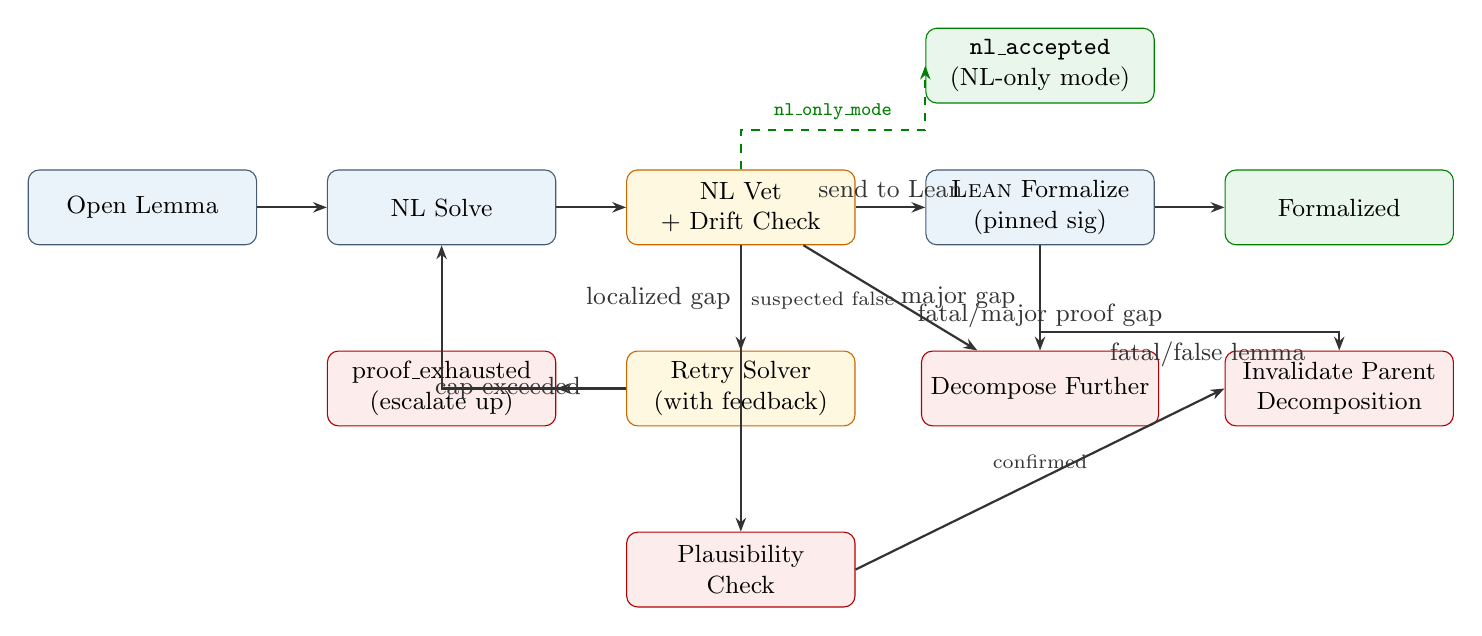
\begin{tikzpicture}[
  every node/.style={font=\small},
  state/.style={rectangle,rounded corners=4pt,draw=deepblue!80,fill=softblue,minimum width=2.9cm,minimum height=0.95cm,align=center},
  warn/.style={rectangle,rounded corners=4pt,draw=orange!80!black,fill=softyellow,minimum width=2.9cm,minimum height=0.95cm,align=center},
  good/.style={rectangle,rounded corners=4pt,draw=green!50!black,fill=softgreen,minimum width=2.9cm,minimum height=0.95cm,align=center},
  bad/.style={rectangle,rounded corners=4pt,draw=red!70!black,fill=softred,minimum width=2.9cm,minimum height=0.95cm,align=center},
  arr/.style={-{Stealth[length=5pt]},thick,color=darkgray}
]
\node[state] (open) at (0,0) {Open Lemma};
\node[state] (solve) at (3.8,0) {NL Solve};
\node[warn] (vet) at (7.6,0) {NL Vet\\+ Drift Check};
\node[state] (lean) at (11.4,0) {\Lean{} Formalize\\(pinned sig)};
\node[good] (done) at (15.2,0) {Formalized};

\node[good] (nldone) at (11.4,1.8) {\texttt{nl\_accepted}\\(NL-only mode)};

\node[warn] (retry) at (7.6,-2.3) {Retry Solver\\(with feedback)};
\node[bad] (decomp) at (11.4,-2.3) {Decompose Further};
\node[bad] (plaus) at (7.6,-4.6) {Plausibility\\Check};
\node[bad] (invalidate) at (15.2,-2.3) {Invalidate Parent\\Decomposition};
\node[bad] (exhausted) at (3.8,-2.3) {proof\_exhausted\\(escalate up)};

\draw[arr] (open) -- (solve);
\draw[arr] (solve) -- (vet);
\draw[arr] (vet) -- node[above]{send to Lean} (lean);
\draw[arr] (lean) -- (done);
\draw[arr,dashed,color=green!50!black] (vet.north) -- ++(0,0.5) -| node[pos=0.25,above,font=\scriptsize,color=green!50!black]{\texttt{nl\_only\_mode}} (nldone.west);
\draw[arr] (vet) -- node[left]{localized gap} (retry);
\draw[arr] (retry.west) -| (solve.south);
\draw[arr] (vet) -- node[right]{major gap} (decomp);
\draw[arr] (vet.south) -- ++(0,-0.7) -| (plaus.north) node[pos=0.2,right,font=\scriptsize]{suspected false};
\draw[arr] (plaus.east) -- node[above,font=\scriptsize]{confirmed} (invalidate.west);
\draw[arr] (lean.south) -- ++(0,-0.6) -| node[pos=0.25,below]{fatal/major proof gap} (decomp.north);
\draw[arr] (lean.south) -- ++(0,-1.1) -| node[pos=0.28,below]{fatal/false lemma} (invalidate.north);
\draw[arr] (retry) -- node[left]{cap exceeded} (exhausted);
\end{tikzpicture}%
}
\caption{Lemma lifecycle. The dashed green path shows the NL-only mode shortcut where vetter acceptance is terminal.}
\end{figure}

%% ═══════════════════════════════════════════════════════════════════════════════
\section{Conclusion}
%% ═══════════════════════════════════════════════════════════════════════════════

This document specifies everything the orchestrator engineer needs to build, test, and deploy the Orthosolver NL pipeline. The \Lean{} engine is treated as a black-box service accessed through the API contract in Section~\ref{sec:lean_api}. During Phase~1, the NL pipeline can be developed and tested end-to-end in NL-only mode with no \Lean{} dependency. The mock service (Section~\ref{sec:lean_mock}) enables testing of standard-mode code paths before the real engine exists. The integration seam is the HTTP contract; once the real \Lean{} engine implements that contract, the merge is a URL swap.

\end{document}
